% !TEX root =  paper.tex

\begin{figure*}[t!]
	\centering
	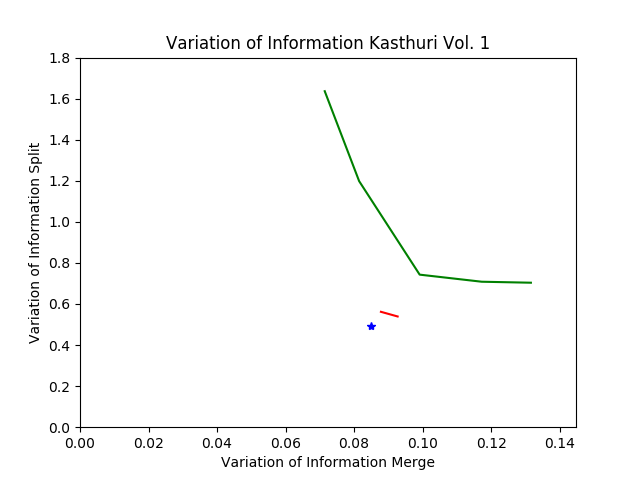
\includegraphics[width=0.45\linewidth]{./figures/variation_of_information-microns-train-600.png}
	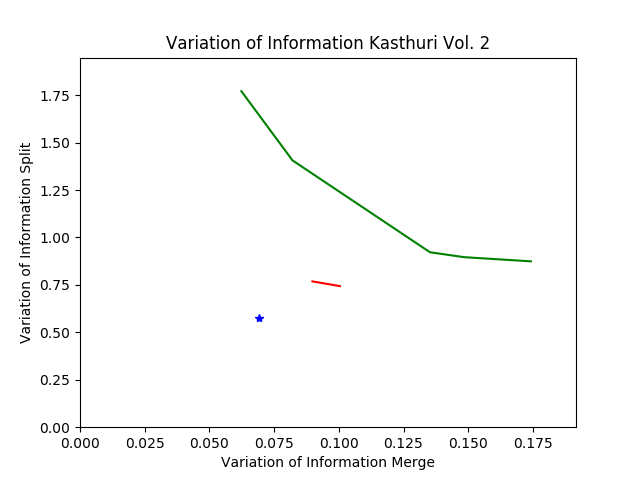
\includegraphics[width=0.45\linewidth]{./figures/variation_of_information-microns-test-600.png}
	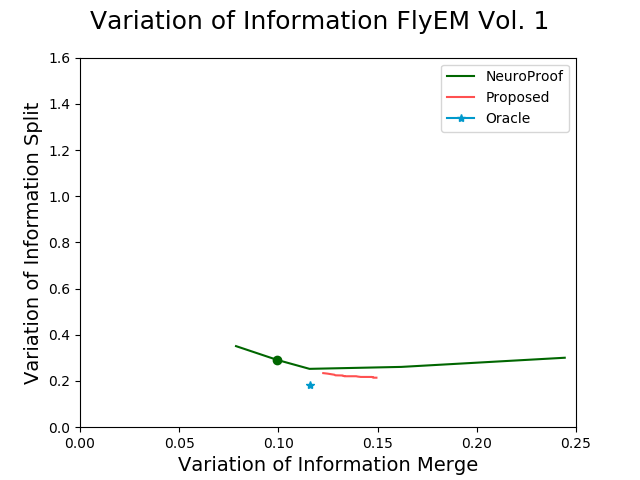
\includegraphics[width=0.45\linewidth]{./figures/variation_of_information-FlyEM-train-600.png}
	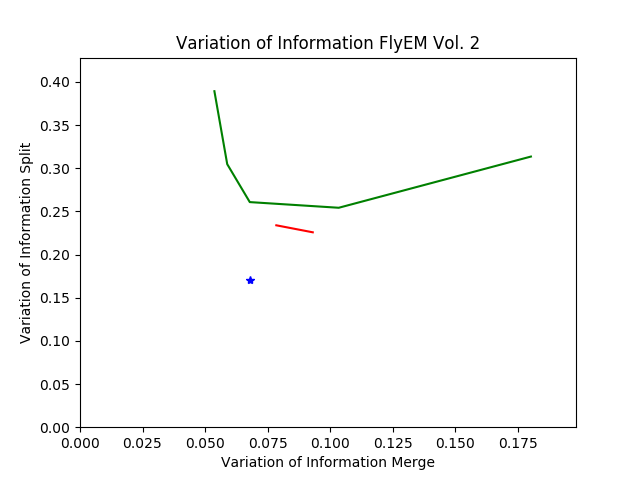
\includegraphics[width=0.45\linewidth]{./figures/variation_of_information-FlyEM-test-600.png}
	\caption{VI scores of our method (red) compared to the baseline segmentation (green) and an oracle (blue) that optimally partitions the graph based on ground truth.}
	\label{fig:variation-of-information}
\end{figure*}

%\section{Results}

\subsection{Error Metric}
\label{sec:variation-of-information}

We evaluate the performance of the different methods using the split version of variance of information (VI)~\cite{meila2003comparing}.
Given a ground truth labeling $GT$ and our automatically reconstructed segmentation $SG$, over and undersegmentation are quantified by the conditional entropy $H(GT | SG)$ and $H(SG | GT)$, respectively. Since we are measuring the entropy between two clusterings, better VI scores are closer to the origin.

\subsection{Variation of Information Results}

In Fig.~\ref{fig:variation-of-information}, we show the VI results of NeuroProof on the Kasthuri and FlyEM data at varying thresholds of agglomeration (green).
The green circle represents the variation of information for our input segmentation with a threshold of 0.3 for all datasets.
Our results are in red.
We show the comparison to an oracle (blue) that correctly partitions the graph from our algorithm based on ground truth.

Our algorithm improves the accuracy of the input segmentation on every dataset, reducing the VI split score on average by \FIX{X\%} and only increasing the VI merge score by \FIX{X\%}.
Scores closer to the origin are better for this metric, and in every instance we are below the green curve.
We see significant improvements on the Kasthuri datasets (VI split reduction of \FIX{X\%} and \FIX{X\%} on the training and testing datasets respectively) and slightly more modest improvements on the FlyEM datasets (reduction of \FIX{X\%} and \FIX{X\%}).
However, our baseline, NeuroProof performs much better on the FlyEM datasets reducing the potential improvement.
Isotropic datasets are easier to segment using state-of-the-art region-based methods than anisotropic ones~\cite{plaza2014annotating}.
Thus there is less room for improvement on these datasets.

Fig.~\ref{fig:positive-results} shows successful merges on the Kasthuri Vol. 2 dataset.
Several of these examples combine multiple consecutive segments that span the volume.
In the third example we correct the oversegmentation of a dendrite.
Fig.~\ref{fig:negative-results} shows some failure cases.
In two of these examples the algorithm correctly predicted several merges but made one error.
In the third example a merge error in the initial segmentation propagated to our output.
We now analyze how each major component of our method contributes to this final result.

\begin{figure}[t]
	\centering
	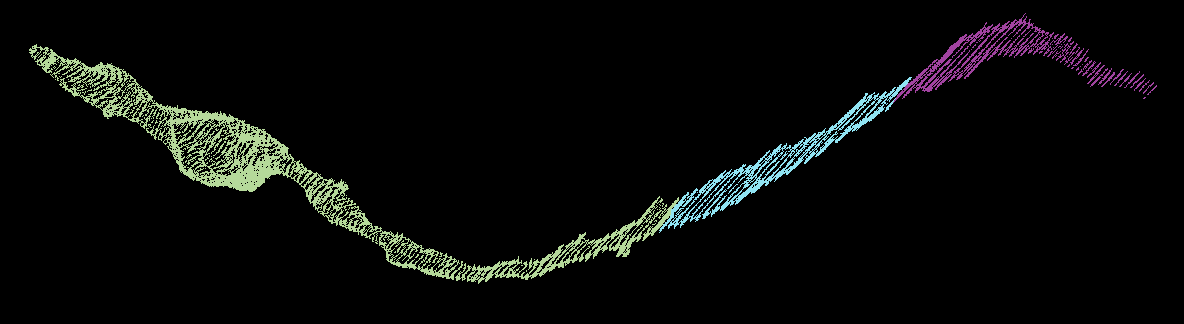
\includegraphics[width=0.85\linewidth]{./figures/multicut-correct1.png}
	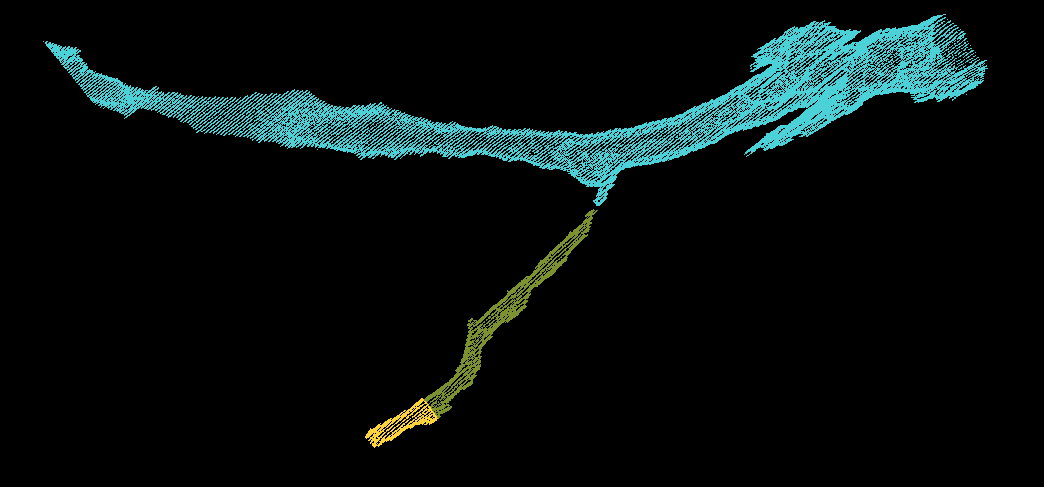
\includegraphics[width=0.85\linewidth]{./figures/multicut-correct2.png}
	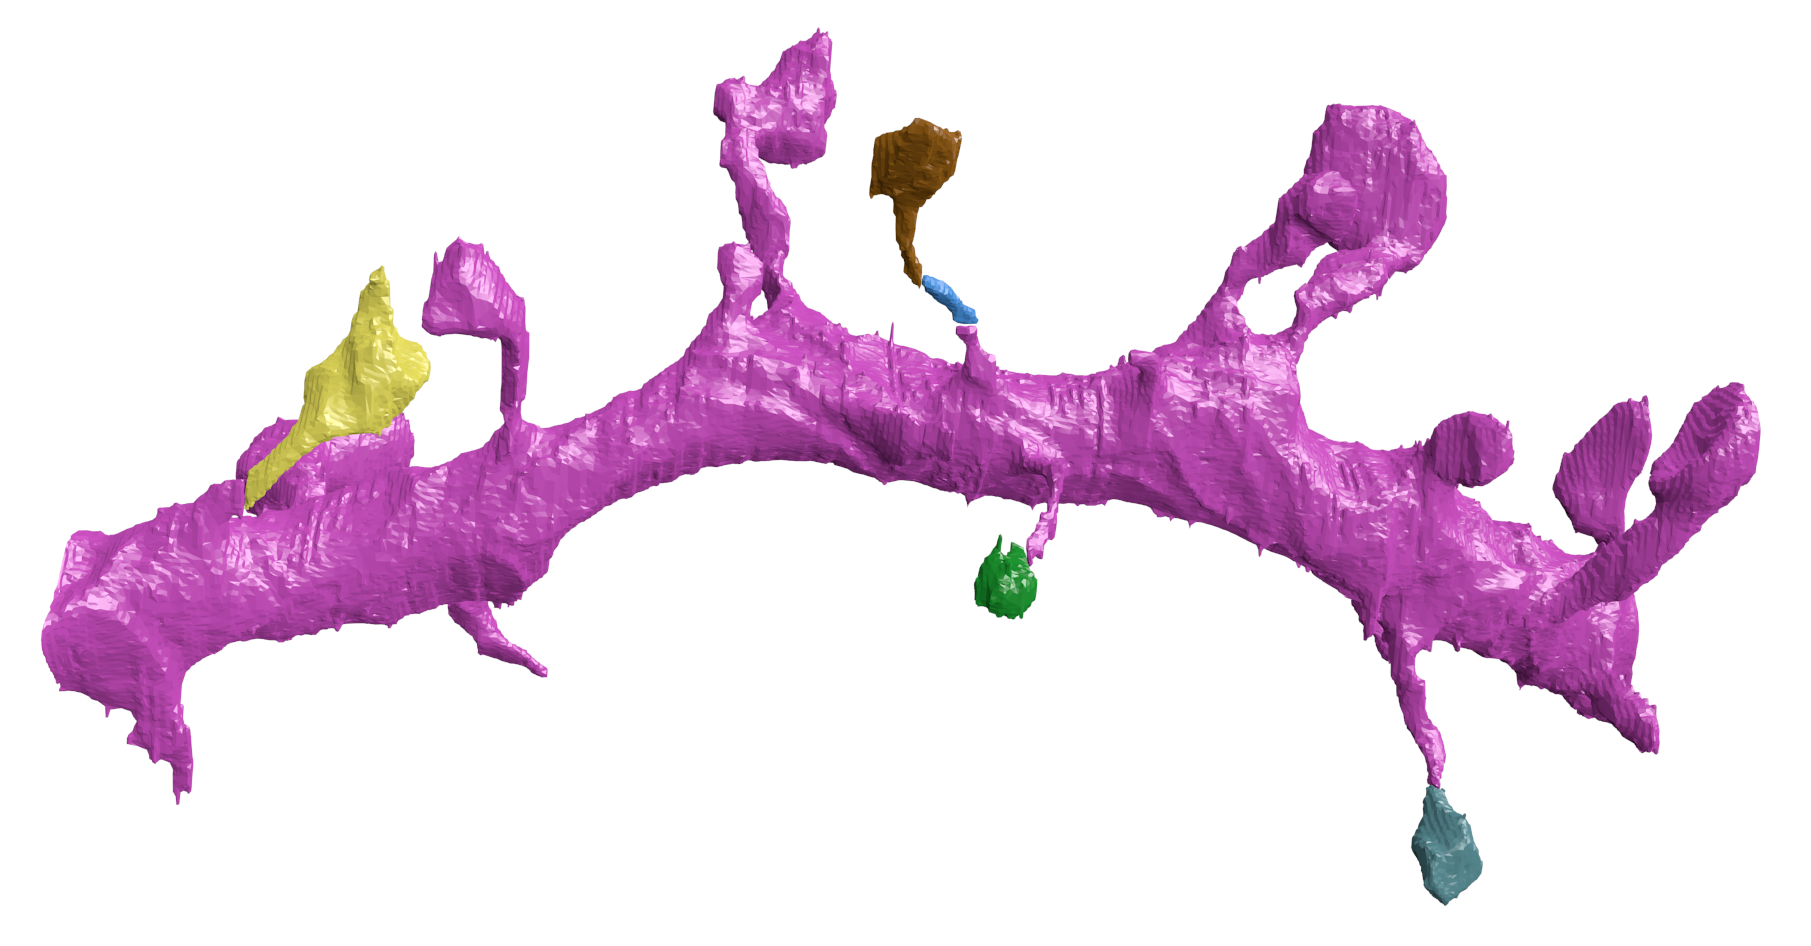
\includegraphics[width=0.85\linewidth]{./figures/multicut-correct3.png}
	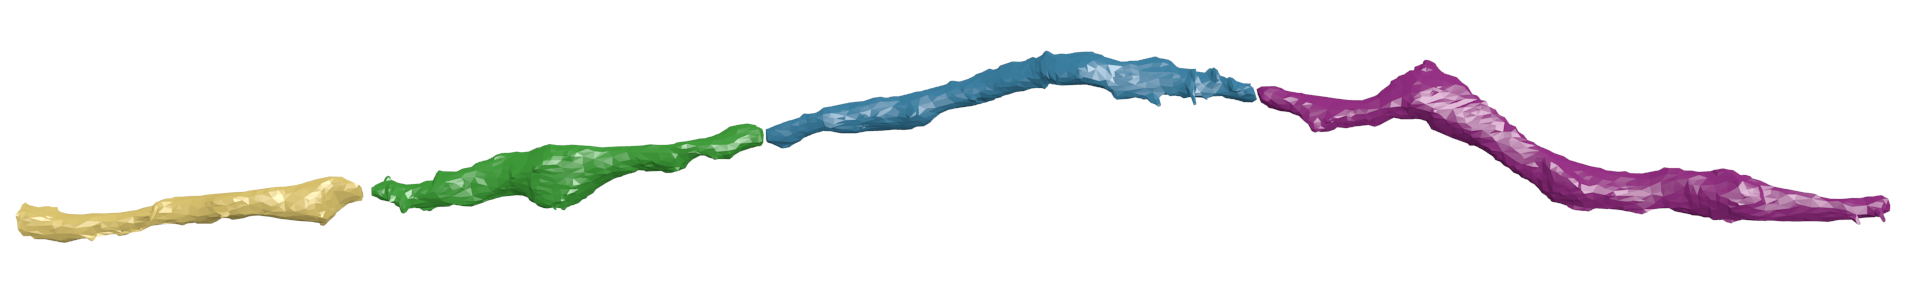
\includegraphics[width=0.85\linewidth]{./figures/multicut-correct4.png}
	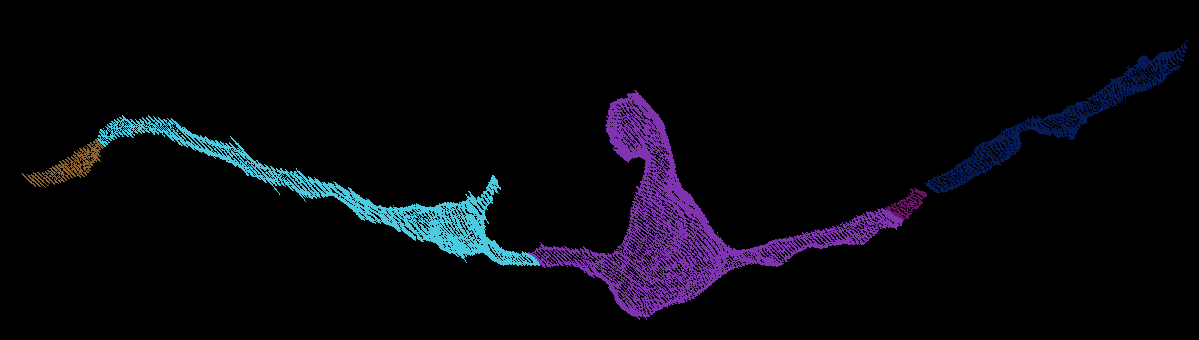
\includegraphics[width=0.85\linewidth]{./figures/multicut-correct5.png}
	\caption{Correctly segmented neurons from our method.}
	\label{fig:positive-results}
\end{figure}

\begin{figure}[t]
	\centering
	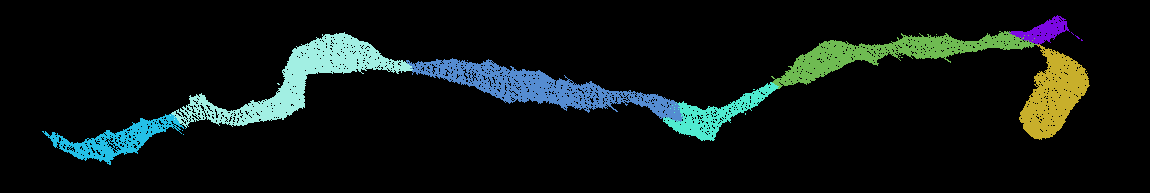
\includegraphics[width=0.85\linewidth]{./figures/multicut-incorrect1.png}
	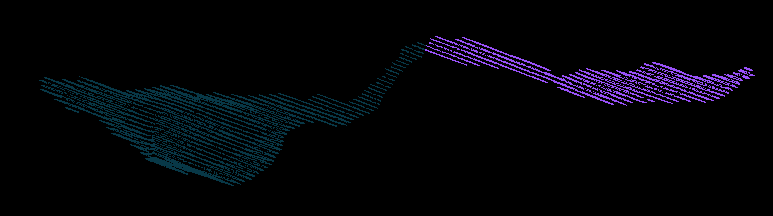
\includegraphics[width=0.85\linewidth]{./figures/multicut-incorrect2.png}
	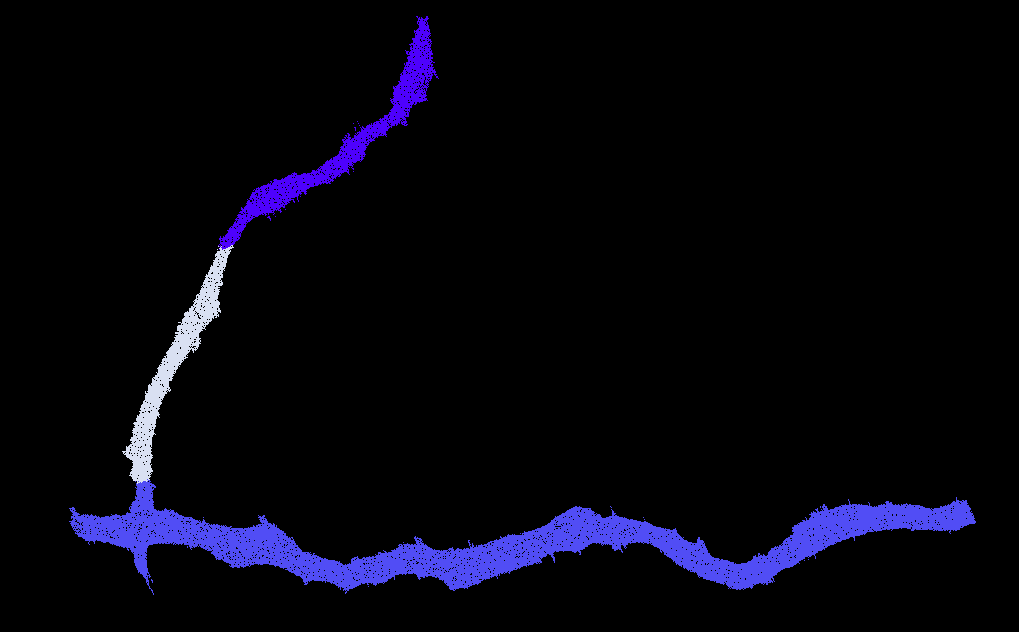
\includegraphics[width=0.85\linewidth]{./figures/multicut-incorrect3.png}
	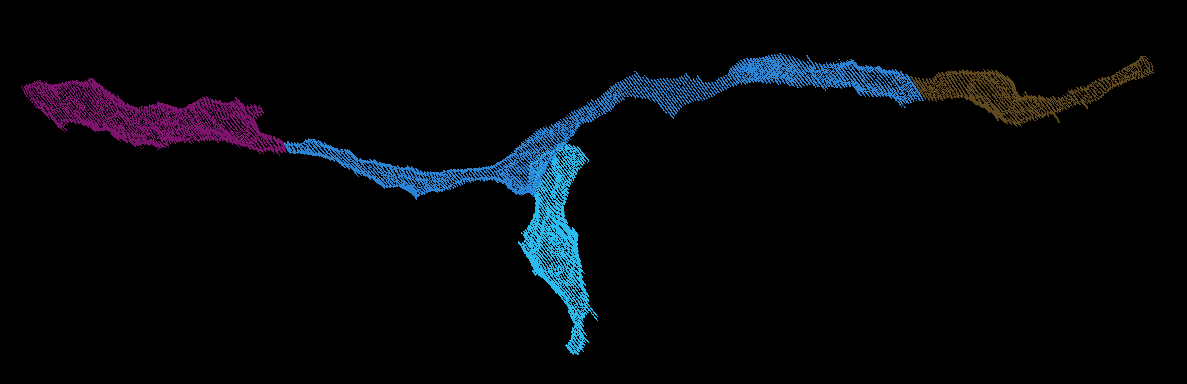
\includegraphics[width=0.85\linewidth]{./figures/multicut-incorrect4.png}
	\caption{Errors made by our method.}
	\label{fig:negative-results}
\end{figure}


\subsection{Graph Creation}

\begin{table}
	\centering
	\small
	\begin{tabular}{c c c} \hline
		\textbf{Dataset} & \textbf{Baseline} & \textbf{After Pruning} \\ \hline
		Kasthuri Vol. 1 & 763 / 21242 (3.47\%) & 753 / 3459 (17.88\%) \\
		Kasthuri Vol. 2 & 1010 / 26073 (3.73\%) & 904 / 4327 (17.28\%) \\
		FlyEM Vol. 1 & 269 / 14875 (1.78\%) & 262 / 946 (21.69\%) \\
		FlyEM Vol. 2 & 270 / 16808 (1.58\%) & 285 / 768 (27.07\%)\\ \hline
	\end{tabular}
	\caption{The results of our skeleton graph pruning heuristic compared to the baseline segmentation.}
	\label{table:skeletonization}
\end{table}

Table \ref{table:skeletonization} shows the results of pruning the skeleton graph using the heuristic discussed in Sec.~\ref{sec:skeletonization}. The baseline algorithm considers all adjacent regions for merging. Our method removes a significant portion of these candidates while maintaining a large number of the true merge locations. This edge pruning is essential for the graph partitioning algorithm, which has a computational complexity dependence on the number of edges. Our pruning heuristic removes at least $6\times$ the number of edges between correctly split segments on all datasets, achieving a maximum removal ratio of $20\times$.

Equally important is the number of split errors that remain after pruning. These are the locations that we want to merge to create a more accurate reconstruction. For every dataset, the number of true split errors remains constant before and after pruning.
However, since our heuristic does not enforce an adjacency constraint of two regions when constructing edges in the graph, the difference does not indicate the number of examples excluded by pruning. In fact, our method finds a number of examples that are non-adjacent. Figure \ref{fig:skeleton-results} shows two example segments with split errors, one that our algorithm missed (top) and one that it identified (bottom), despite the fact that the split segments are not adjacent.
Of the successful examples in Figure \ref{fig:positive-results}, the second and fourth groupings contain pairs of non-adjacent segments that merge with our algorithm.

\begin{figure}[h!]
	\centering
	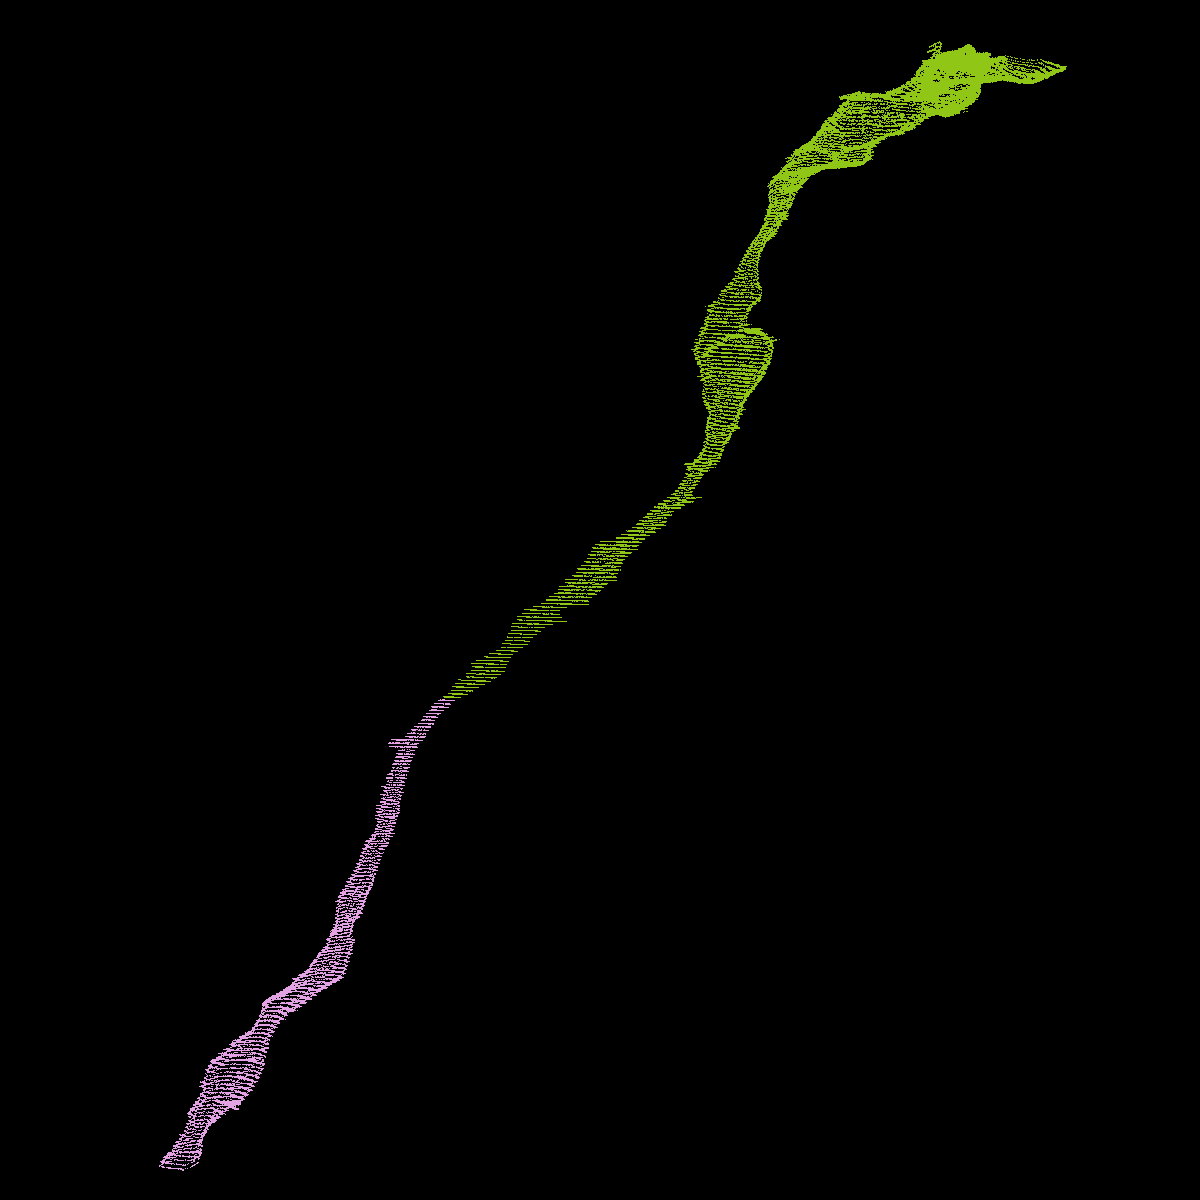
\includegraphics[width=0.85\linewidth]{./figures/merge_candidate1.png}
	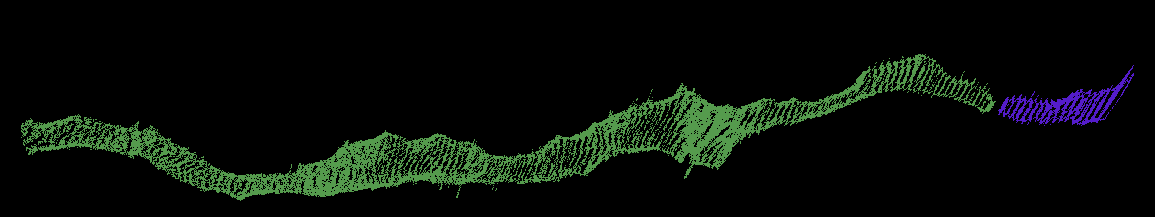
\includegraphics[width=0.85\linewidth]{./figures/merge_candidate2.png}
	\caption{Example merge candidates.}
	\label{fig:skeleton-results}
\end{figure}


\subsection{Classification Performance}

Figure \ref{fig:receiver-operating-characteristic} shows the receiver operating characteristic (ROC) curve for all of the datasets.
We train our CNN using one of the Kasthuri volumes and test using the other three datasets.
Since our CNN only takes as input a region of the label volume we can train on an anisotropic dataset and infer on an isotropic one.
This provides a major benefit given the time-intensive task of manually generating ground truth data at various resolutions.

As evidenced by the ROC curve, the test results on the Kasthuri data are better than the results for FlyEM.
We believe this is in part because of the differences in the datasets (i.e., isotropy and $xy$ resolution).
To test this hypothesis, we also evaluate the performance of the FlyEM datasets when the network trains on FlyEM Vol. 1 and infers on FlyEM Vol. 2.\footnote{Since the FlyEM datasets have significantly fewer examples, we initialize the network with the weights from the Kasthuri training and have an initial learning rate of $10^{-4}$.}
The dotted lines in the figure represent these tests.
There is a slight performance increase for FlyEM Vol. 2.
However, the FlyEM datasets have reasonable results when the network is trained by the Kasthuri data, and the results outside of this section follow from that setup.

\begin{figure}
	\centering
	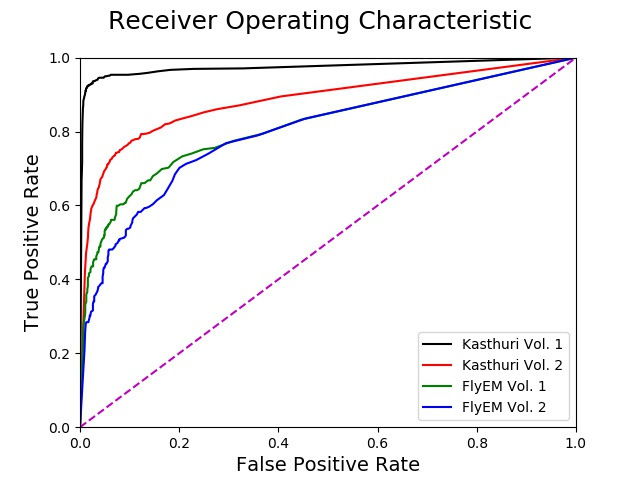
\includegraphics[width=0.95\linewidth]{./figures/receiver-operating-characteristic.jpg}
	\caption{The receiver operating characteristic for all four datasets.}
	\label{fig:receiver-operating-characteristic}
\end{figure}

\subsection{Graph Based Strategies}

The graph-based optimization strategy increases our correction accuracy over using just the CNN.
In particular, the precision increases on each dataset, although the recall decreases on all but one of the datasets.
Since it is more difficult to correct merge errors than split errors, it is often desirable to sacrifice recall for precision.
Table \ref{table:multicut} shows the changes in precision, recall, and accuracy for all four datasets compared to the CNN.
Over the three testing datasets, applying a graph-based partitioning strategy reduced the number of merge errors by \FIX{X}, \FIX{Y}, and \FIX{Z}.

\begin{table}[h]
	\centering
	\begin{tabular}{c c c c} \hline
		\textbf{Dataset} & $\Delta$ \textbf{Precision} & $\Delta$ \textbf{Recall} & $\Delta$ \textbf{Accuracy} \\ \hline
		Kasthuri Training & +3.60\% & -0.01\% & +0.60\% \\
		Kasthuri Testing & +7.59\% & -1.77\% & +1.38\% \\
		FlyEM Vol. 1 & +2.68\% & +0.76\% & +0.66\% \\
		FlyEM Vol. 2 & +2.22\% & -1.05\% & +0.29\% \\ \hline
	\end{tabular}
	\caption{Precision and recall for the training and three test datasets.}
	\label{table:multicut}
\end{table}
